\begin{figure*}[htbp]
    % \centering
    \hspace*{-2cm}
    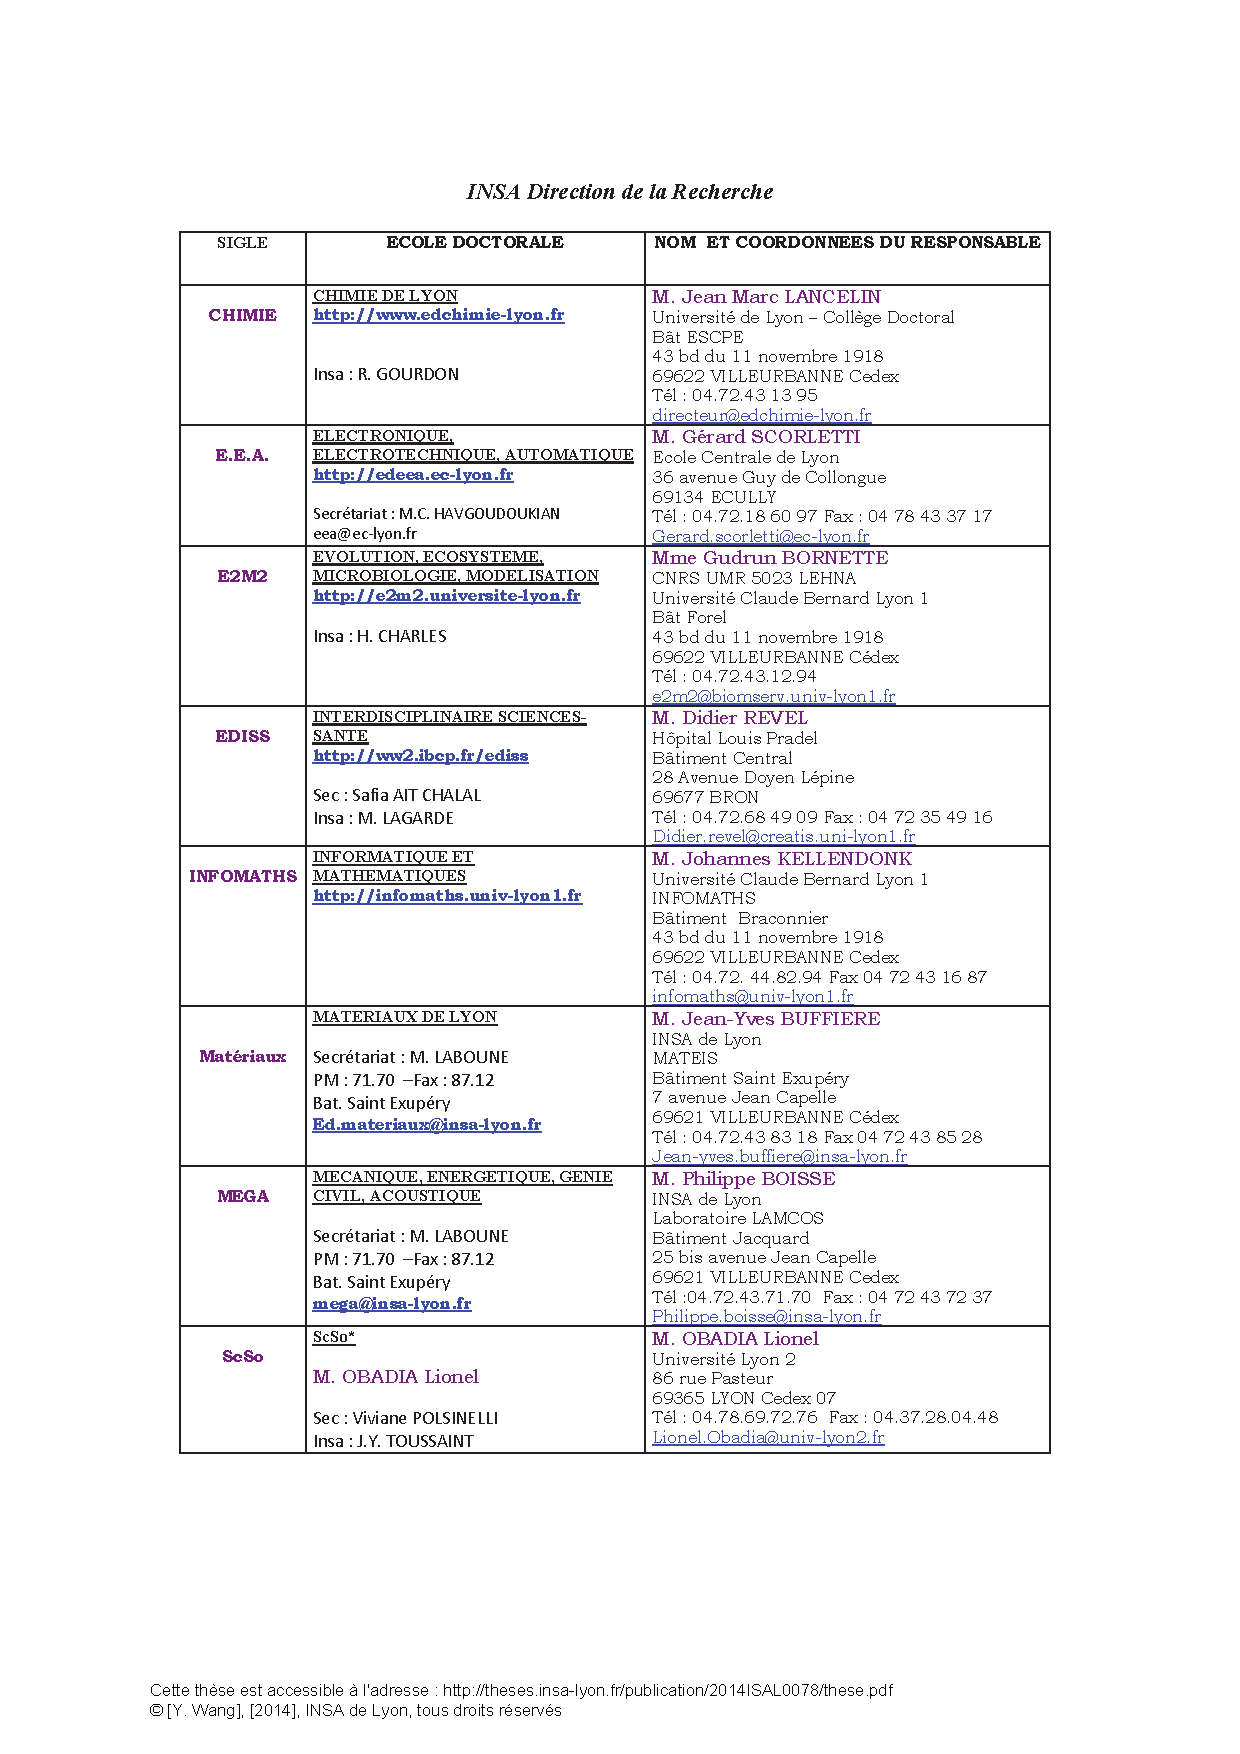
\includegraphics[trim=0cm 0cm 0cm 2.8cm, clip, width=1.30\textwidth]{gfx/ED.pdf} %% UGLY HACK because I don't want to rewrite by hand this unaesthetic document : http://www.insa-lyon.fr/sites/www.insa-lyon.fr/files/ecoles-doctorales_2011-2015_maj12102015.pdf
\end{figure*}

\clearpage

%% Folio administratif : http://www.insa-lyon.fr/sites/www.insa-lyon.fr/files/folio.doc

\includegraphics[height=1.5cm]{gfx/Logo_INSALyon}

{
\begin{center}
  \textsc{Folio administratif}\\
  \textsc{Thèse soutenue devant l'Institut National des Sciences Appliquées de Lyon}
\end{center}
}
\vfill

{
\setlength{\tabcolsep}{0pt}
\newenvironment{entrylist}{%
  \begin{tabular*}{\textwidth}{@{}p{.5\textwidth}l@{}}
}{%
  \end{tabular*}
}
% \renewcommand{\bfseries}{\headingfont\color{headercolor}}
\newcommand{\entry}[2]{%
  #1 & #2%
  \\}
\newcommand{\entryMerged}[1]{%
  \multicolumn{2}{p{\textwidth}}{#1}%
  \\}
\newcommand{\entryEmpty}[0]{%
  &%
  \\}

\begin{entrylist}
  \entry
    {\textsc{Nom :} Levallois}
    {\textsc{Date de Soutenance :} 12/11/2015 }
  \entry
    {\textsc{Prénoms :} Jérémy, Nicolas}
    {}
  \entryEmpty
  \entryMerged
    {\textsc{Titre :} Estimateurs différentiels en géométrie discrète : applications à l'analyse de surfaces digitales}
  \entryEmpty
  \entry
    {\textsc{Nature :} Doctorat}
    {\textsc{Numéro d'ordre :} \thesisOrderNumber}
  \entryMerged
    {\textsc{École Doctorale :} InfoMaths ED 512}
  \entryMerged
    {\textsc{Spécialité :} Informatique}
  \entryEmpty
  \entryMerged
    {\textsc{Résumé :} voir page \pageref{sec:abstract-french}}
  \entryMerged
    {\textsc{Mots-clés :} \emph{géométrie discrète; convergence asymptotique; quantités differentielles; courbure; normales; estimateurs; invariants par intégration; points caractéristiques; classification de surface;}}
  \entryEmpty
  \entryMerged
    {\textsc{Laboratoire(s) de recherche :} LIRIS, LAMA}
  \entryMerged
    {\textsc{Directeur(s) de thèse :} \thesisFirstSupervisor, \thesisSecondSupervisor}
  \entryMerged
    {\textsc{Président de jury :} Nicolas Passat}
  \entryMerged
    {\textsc{Composition du jury :}}
  \entry
    {Nicolas Passat}
    {Président du jury}
  \entry
    {Pierre Alliez}
    {Rapporteur}
  \entry
    {Éric Andrès}
    {Rapporteur}
  \entry
    {Yan Gérard}
    {Examinateur}
  \entry
    {Simon Masnou}
    {Examinateur}
  \entry
    {\thesisFirstSupervisor}
    {Directeur de thèse}
  \entry
    {\thesisSecondSupervisor}
    {Directeur de thèse}
\end{entrylist}
}

\vfill
